\documentclass[xcolor={svgnames}]{beamer}
\usetheme[
numbering=fraction, % curr_page / total_page
block=fill,         % 为 block 显示方框
% progressbar=frametitle % add a progressbar at frametitle
sectionpage=progressbar
]{metropolis}

%% 保留熟悉的数学字体:两种方法
% \usefonttheme[onlymath]{serif}
\renewcommand\mathfamilydefault{\rmdefault}


\input ../defs.tex  % some frequently used alias


\usepackage[english]{babel}
% \usepackage{enumitem} % 支持自定义 item symbol
\usepackage{tikz}
\usetikzlibrary{tikzmark,positioning,shapes,calc}
\usepackage{mathtools}
\usepackage{fancybox} %支持文本框
\usepackage{subfig} %支持subfig
\usepackage{cite}
%\usepackage{biblatex}
%\usepackage[backend=biber,style=numeric-comp,sorting=none]{biblatex}
%\addbibresource{int-ref.bib}

% Removes icon in bibliography
\setbeamertemplate{bibliography item}[text]

% add following for otherwise it will complain
% see https://tex.stackexchange.com/questions/426088/texlive-pretest-2018-beamer-and-subfig-collide
\makeatletter
\let\@@magyar@captionfix\relax
\makeatother
%%%

%=== font customization ===%
%%
%% Note that once use customizing fonts, switch to xelatex
%%
% \usepackage{fontenc}
% \setsansfont{Varela Round}
% % \setsansfont{IM FELL DW Pica}
% \setmonofont{DejaVu Sans Mono}
% \setmathfont{Fira Sans}


% % 目录标数字
\setbeamertemplate{section in toc}[sections numbered]
% % 无序列表用实心点
% \setbeamertemplate{itemize item}{$\bullet$}
% \setbeamertemplate{navigation symnols}{}

%% 设置列表的 item symbol
\setbeamertemplate{itemize item}{\textbullet}
\setbeamertemplate{itemize subitem}{$\blacktriangleright$}
\setbeamertemplate{itemize subsubitem}{$\checkmark$}

%% 定理环境计数
\setbeamertemplate{theorems}[numbered]
% \setbeamertemplate{lemmas}[numbered]

% 定义颜色
\definecolor{alizarin}{rgb}{0.82, 0.1, 0.26} % 红色
\definecolor{DarkFern}{HTML}{407428}         % 绿色
\definecolor{tyorange}{HTML}{ff6600}
\definecolor{tyblue}{HTML}{0066ff}
\colorlet{main}{DarkFern!100!white}          % 第一种设置方法
\colorlet{main}{red!70!black}                % 第二种设置方法
\definecolor{bistre}{rgb}{0.24, 0.17, 0.12}  % 黑色
\definecolor{mygrey}{rgb}{0.52, 0.52, 0.51}  % 灰色
\colorlet{main}{tyblue}
\colorlet{text}{bistre!100!white}

% 不同元素指定不同颜色,fg是本身颜色,bg是背景颜色,!num!改变数值提供渐变色
% \setbeamercolor{title}{fg=main}
% \setbeamercolor{frametitle}{fg=main}
% \setbeamercolor{section in toc}{fg=text}
% \setbeamercolor{normal text}{fg=text}
% \setbeamercolor{block title}{fg=alizarin,bg=mygrey!20!white}
% \setbeamercolor{block body}{fg=black,bg=mygrey!15!white}
% \setbeamercolor{qed symbol}{fg=main} % 证明结束后的框颜色
% \setbeamercolor{math text}{fg=black}

%=== set theme background color to white ===%
% \setbeamercolor{background}{bg=black}
\setbeamercolor{alerted text}{fg=red!50!black}
\setbeamercolor{normal text}{fg=black!85!}
\setbeamercolor{example text}{fg=black!50!cyan}
% \setbeamercolor{frametitle}{bg=Grey}



%-------------------正文-------------------------%

\title{Interpretability of Deep Learning}
\subtitle{(draft)}
\author{Bingbing Hu}
\institute{SIST, ShanghaiTech}
\date{\today}

\begin{document}

\frame[plain,noframenumbering]{\titlepage}

%=== index page ===%
\begin{frame}{Outline}
\tableofcontents
\end{frame}

%=== begin your slides ==%
\section{Motivation}
% 生成当前 section 的 outline page
% \frame{\frametitle{Outline}\tableofcontents[currentsection]}

\begin{frame}{Motivation}
	\begin{figure}[htbp]
		\centering
		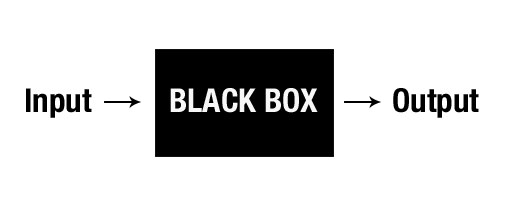
\includegraphics[width=0.7\textwidth]{figures/blackbox.jpg}
	\end{figure}
\end{frame}
%%%%%%%%%%%%%%%%%%%%%%%%%%%%%%%%%%%%%%%%%%%%%%%%%%%%%%%%%%%%%
\begin{frame}{Motivation}
	\begin{itemize}
		\item Deep Learning (DL) is hot but quite a blackbox
		\item Interpretability is demanding \\
			self-driving car, healthcare, criminal justice ...
		\item Why shall we trust it
	\end{itemize}
	We should understand \& be able to reason about model output.
\end{frame}
%%%%%%%%%%%%%%%%%%%%%%%%%%%%%%%%%%%%%%%%%%%%%%%%%%%%%%%%%%%%%
\begin{frame}{Notion of Interpretability}
	\begin{itemize}
			\item Model transparency
				\begin{itemize}
						\item simulatability
						\item decomposability
						\item algorithm transparency
				\end{itemize}
			\item Model functionality
				\begin{itemize}
						\item textual description
						\item visualization
						\item local explanation
				\end{itemize}			
	\end{itemize}
\end{frame}

\section{Interpretability}

\subsection{Model Transparency}

\begin{frame}{Model Transparency}
	\only<1>{
		\footnote{Erhan et al., University of Montreal, 2009}Visualizing the response of individual units in unsupervised deep belief networks\cite{erhan2009visualizing}.
		\begin{itemize}
			\item analyze units in any layer
			\item \footnote{Zeiler et al., ECCV, 2014}extended by \cite{zeiler2014visualizing} to supervised CNN for higher-layer analysis
			\item visualize to guide modifications
		\end{itemize}
	}
	\only<2>{
		\footnote{Mahendran et al., Proceedings of CVPR, 2015}Investigate information in different layer\cite{mahendran2015understanding}.	
		\begin{itemize}
			\item investigate image representation at different CNN layers
			\item reval deeper layers learn more abstract representation of a image
		\end{itemize}
	}
	\only<3>{
		\footnote{Simonyan et al., arXiv preprint, 2013}Generate model-preferred inputs\cite{simonyan2013deep}.
		\begin{itemize}
			\item generate images by maxmizing output score
			\item qualitatively demonstrate the features most representation each class
		\end{itemize}
	}
	\only<4>{
		\footnote{Nguyen et al., arXiv preprint, 2016}Generate perferred images to particular neurons in CNN\cite{nguyen2016multifaceted}.
		\begin{itemize}
			\item use Deep Generator Network to generate images
			\item producing very realistic images 
			\item try to understand what the network has learned
		\end{itemize}
	}
	\only<5>{
		\footnote{Koh et al., arXiv preprint, 2017}How a model's predictions would differ if a data point were altered, or not seen during training\cite{koh2017understanding}?
		\begin{itemize}
			\item use statistical influence functions to approximate the disturb of data points without retrain the model
			\item assess the importance of particular training point
			\item generate adversarial examples to attack the trained model
		\end{itemize}
	}
	\only<6>{
		\footnote{Shwartz-Ziv et al., arXiv preprint, 2017}Analyze deep networks using \alert{information theory}\cite{shwartz2017opening}.
		\begin{itemize}
			\item calculate how info. is preserved on each layer's in/out-puts
			\item learn how SGD optimizes the network
			\item the depth of the network is consistent with IB optimality
		\end{itemize}
	}
\end{frame}

\subsection{Model Functionality}

\begin{frame}{Model Functionality}
	Model functionality can be explained by post-hoc interpretations of what the model has done.
		\begin{itemize}
			\item Using t-SNE to visualize model output
			\item \ldots \ldots
		\end{itemize}
\end{frame}
 
%%%%%%%%%%%%%%%%%%%%%%%%%%%%%%%%%%%%%%%%%%%%%%%%%%%%%%%%%%%%%

\section{Information Bottleneck}

\begin{frame}
	\only<1>{
	Deep Learning and the Information Bottleneck Principle \\
	(Naftali TIshby \& Noga Zaslavsky)
	}
	\begin{figure}[hp]
		\centering
		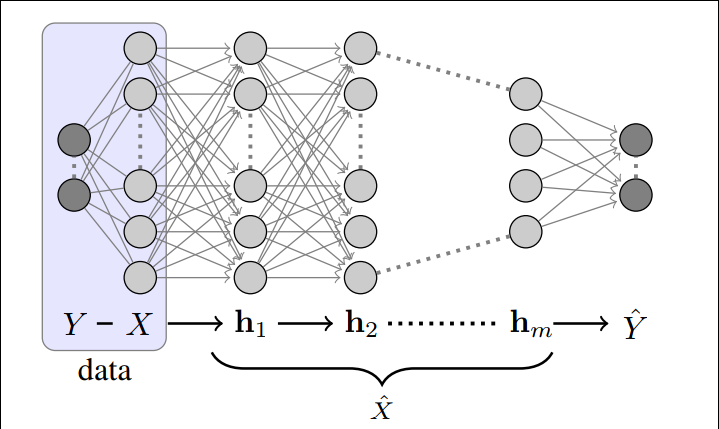
\includegraphics[width=0.8\textwidth]{figures/dnn.png}
	\end{figure}
	\only<2>{
		\begin{align*}
			X: &\text{ input, low-level representation of data} \\
			Y: &\text{ desired output, lower dimension}
		\end{align*}
		The most entropy of $X$ is not very informative about $Y$.
	}
\end{frame}
%%%%%%%%%%%%%%%%%%%%%%%%%%%%%%%%%%%%%%%%%%%%%%%%%%%%%%%%%%%%%
\begin{frame}{IB Principle}
	Given input $X \in \mathcal{X}$, output $Y \in \mathcal{Y}$, we want to compress $X$ while preserve the information about $Y$. 
\pause

	An optimial representation will compress $X$ by dismissing the irrelevant parts which give no info. about $Y$.
\pause
\bigskip	
	\begin{exampleblock}{Summary}
		Namely, find the relevant parts $\hat{X}$ inside $X$ w.r.t. $Y$ to minimize
		\[
			\mathcal{L}[p(\hat{x}|x)] = I\left( X;\hat{X} \right) - \beta I\left( \hat{X};Y \right)
		\]
	\end{exampleblock}
\end{frame}
%%%%%%%%%%%%%%%%%%%%%%%%%%%%%%%%%%%%%%%%%%%%%%%%%%%%%%%%%%%%%
\begin{frame}{IB vs. Rate-Distortion}
	Rate distortion: $X \in \mathcal{X}$, find a representation $\hat{X}$ of $X$ \\
	Goal: minimize the ``distance between'' $X$ and $\hat{X}$ \\
	\pause
	Need a distance measure: $d_{IB}(x,\hat{x}) = D_{KL}[p(y|x) \| p(y|\hat{x})]$
	$\implies D_{IB} = \E[d_{IB}(x,\hat{x})] = I(X;Y|\hat{X})$
	
	\pause
	To minimize
	\[
		\tilde{\mathcal{L}}[p(\hat{x}|x)] = I\left( X;\hat{X} \right) + \beta I\left( X;Y | \hat{X} \right)
	\]

	Note: $I( X;Y | \hat{X} )$ can be viewed as the relevant information \emph{not} captured by $\hat{X}$.
\end{frame}
%%%%%%%%%%%%%%%%%%%%%%%%%%%%%%%%%%%%%%%%%%%%%%%%%%%%%%%%%%%%%
\begin{frame}{Applied to DNN}
	\begin{figure}[hp]
		\centering
		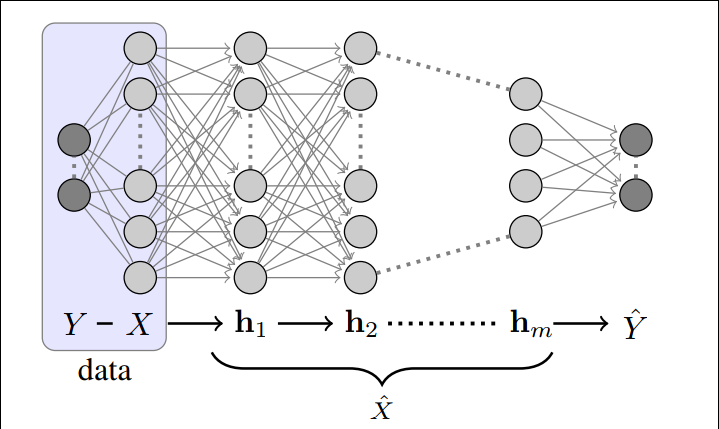
\includegraphics[width=0.6\textwidth]{figures/dnn.png}
	\end{figure}
	\[
		I(Y;X) \ge I(Y;\bd{h}_{i-1}) \ge I(Y;\bd{h}_i) \ge I(Y;\hat{Y})
	\]
	\pause
	At each layer,
	\begin{itemize}
		\item maximize $I(Y;\bd{h}_i)$: view $\bd{h}_i$ as $\hat{X}$
		\item minimize $I(\bd{h}_{i-1};\bd{h}_i)$: view $\bd{h}_{i-1}$ as $X$
	\end{itemize}
\end{frame}

%%%%%%%%%%%%%%%%%%%%%%%%%%%%%%%%%%%%%%%%%%%%%%%%%%%%%%%%%%%%%

\begin{frame}{Applied to DNN}
	From $I( X;\hat{X} ) + \beta I( X;Y | \hat{X} )$, by defining $\bd{h}_0 = X$ and $\bd{h}_{m+1} = \hat{Y}$ we get
	\[
		I( \bd{h}_{i-1};\bd{h}_i ) + \beta I( Y;\bd{h}_{i-1} | \bd{h}_i),
	\]
	which gives a optimal rule for training.
\end{frame}

%%%%%%%%%%%%%%%%%%%%%%%%%%%%%%%%%%%%%%%%%%%%%%%%%%%%%%%%%%%%%

\begin{frame}{Applied to DNN}
	However, the joint distribution $p(X,Y)$ is unknown in general!
	\begin{itemize}
		\item representational complexity $K = |\hat{\mathcal{X}}|$
		\item finite sample distribution $\hat{p}(x,y)$
		\item empirical mutual info. $\hat{I}(X,Y)$
	\end{itemize}
	\cite{shamir2010learning} gives
	\[
	\begin{split}
		I\left(\hat{X};Y\right) &\le \hat{I}\left(\hat{X};Y\right) + O\left(\frac{K |\mathcal{Y}|}{\sqrt{n}}\right) \\
		I\left(\hat{X};X\right) &\le \hat{I}\left(\hat{X};X\right) + O\left(\frac{K}{\sqrt{n}}\right)
	\end{split}
	\]
\end{frame}

%%%%%%%%%%%%%%%%%%%%%%%%%%%%%%%%%%%%%%%%%%%%%%%%%%%%%%%%%%%%%

\begin{frame}{Applied to DNN}
	\begin{figure}[hp]
		\centering
		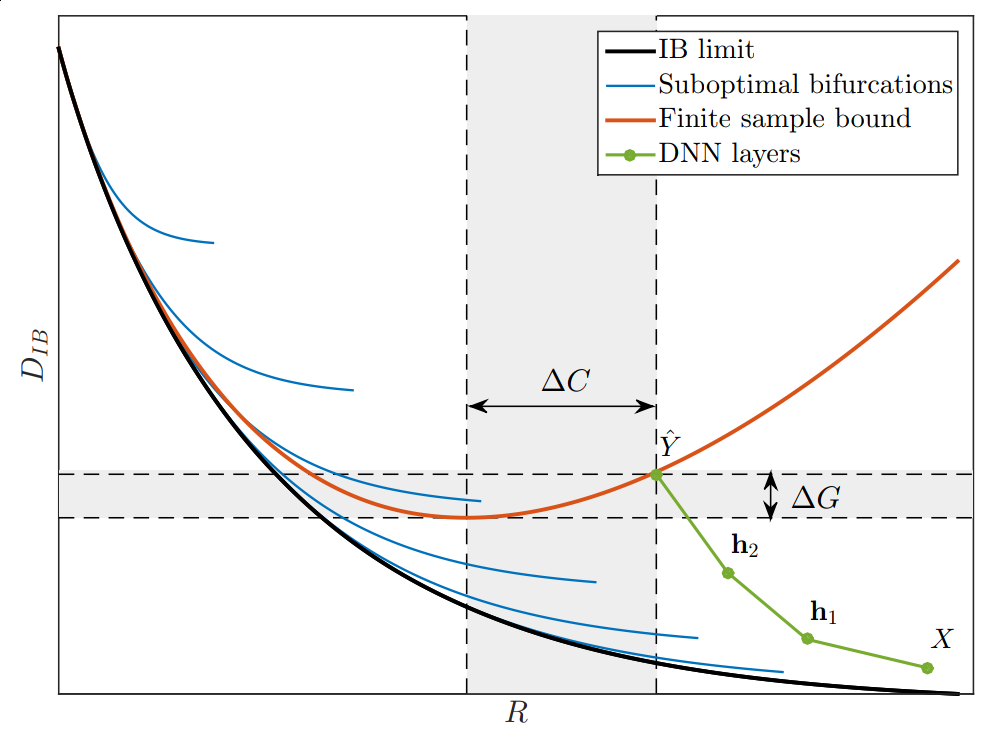
\includegraphics[width=0.7\textwidth]{figures/info-plane.png}
	\end{figure}
\end{frame}

%%%%%%%%%%%%%%%%%%%%%%%%%%%%%%%%%%%%%%%%%%%%%%%%%%%%%%%%%%%%%

\begin{frame}{Applied to DNN}
	Some insight:
	\begin{itemize}
		\item input layer has a bad generalization since it's complexity
		\item hidden layer compressed the input for a better generalization
	\end{itemize}
\end{frame}

%%%%%%%%%%%%%%%%%%%%%%%%%%%%%%%%%%%%%%%%%%%%%%%%%%%%%%%%%%%%%

\begin{frame}[allowframebreaks]{References}
	%\bibliographystyle{plain}
	%\bibliography{int-ref}
	\bibliographystyle{amsalpha}
	\bibliography{./int-ref.bib}
\end{frame}

%%%%%%%%%%%%%%%%%%%%%%%%%%%%%%%%%%%%%%%%%%%%%%%%%%%%%%%%%%%%%

\begin{frame}[standout]
  \Huge Thank you!
\end{frame}

% \begin{frame}[label=conclusion, standout]{Conclusion}
%   Awesome slide
% \end{frame}
\end{document}
